\documentclass[12pt, oneside]{article}

\usepackage[english]{babel}
\usepackage[utf8]{inputenc}
\usepackage{amsmath}
\usepackage{graphicx}
\usepackage[margin=1in]{geometry}

\title{Age of 911 Callers}
\author{Jacob Mortensen}
\date{\today}

\begin{document}
\maketitle
\begin{enumerate}

\item Given that the likelihood is 
$$L(\Lambda) = exp\left\{-\sum_{a=0}^{110}\Lambda(a)\right\}\prod_{i=1}^{N}\Lambda(a_i)$$
If we factor $\Lambda(a) = \delta \lambda(a_i)$ then we can rewrite the likelihood function as
$$ L(\Lambda) = \exp\left\{-\delta\right\}\delta^N\prod_{i=1}^{N}\lambda(a_i)$$
since $\sum_{a=0}^{110}\lambda(a) = 1$.

\item For this problem, I elected to use a Poisson(50) truncated at 110. 
  In order to sum to 1, we need to divide the normal poisson by the sum of the densities 
  from 0 to 110, and when I calculated this in R it turned out to just be 1, so we can 
  just use a normal Poisson as our density for $\lambda(a)$.
 
  With this new value for $\lambda(a)$ our likelihood function becomes:
  $$ L(\delta | a) = exp\left\{-\delta\right\}\delta^N\prod_{i=1}^N\frac{50^{a_i}e^{-50}}{a_i!} $$

\item If we treat $\prod_{i=1}^N\frac{50^{a_i}e^{-50}}{a_i!}$ as a constant then we can see 
  that this likelihood appears to be the kernel of a Gamma($N+1$,$1$) so I propose we use a 
  Gamma(5, 0.2) as the conjugate prior for $\delta$.
 
  If we multiply these together we get 
  \begin{align*}
    exp\left\{-0.2\delta\right\}\delta^{5-1}exp\left\{-\delta\right\}\delta^N
    &= exp\left\{-1.2\delta\right\}\delta^{N+5-1}
  \end{align*}

  We recognize this as the kernel of the Gamma($N+5$, $1.2$) distribution,
  and we see that the Gamma distribution is indeed conjugate to our likelihood. 
  Therefore our posterior density is 
  $$ f(\delta | N+5, 1.2) = \frac{1.2^{N+5}}{\Gamma\left(N+5\right)}exp\left\{-1.2\delta\right\}\delta^{N+5-1} $$

\item Now we let $\lambda(a)$ be the MN(1, $p_0$, $p_1$, \dots, $p_{110}$). Then our likelihood 
  becomes 
  $$ L(\delta|a) = exp\left\{-\delta \right\} \delta^N \prod_{i=1}^N p_{a_i} 
    = exp\left\{-\delta \right\} \delta^N p_0^{N_0}p_1^{N_1}\dots p_{110}^{N_{110}} 
    \propto p_0^{N_0}p_1^{N_1}\dots p_{110}^{N_{110}}
  $$
  We recognize this as the kernel of the Dirichlet distribution and so we propose a 
  symmetric Dirichlet distribution as a conjugate prior for this distribution. Let our 
  density for our prior be 
  $$ f(p_1, p_2, \dots, p_{110} | \alpha) = \prod_{i=1}^{110} p_i^{\alpha-1} $$
  Then multiplying this by our likelihood we get 
  $$ \left(\prod_{i=1}^{110}p_i^{\alpha-1}\right) p_0^{N_0}p_1^{N_1}\dots p_{110}^{N_{110}} 
  = p_0^{\alpha+N_0-1}p_1^{\alpha+N_1-1}\dots p_{110}^{\alpha+N_{110}-1} $$

  We can see that we are again left with the kernel of the Dirichlet distribution 
  and so our posterior distribution for
  $p_1, \dots, p_{110}$ is 
  $$ \frac{\Gamma\left(\sum_{i=1}^{110}\alpha+N_i\right)}{\prod_{i=1}^{110}\Gamma\left(\alpha+N_i\right)} 
  \prod_{i=1}^{110}p_i^{N_i+\alpha-1} $$

\item The plot of the posterior density of $\delta$ and the posterior means of $p_0, \dots, p_{110}$ can be seen in Figures \ref{delta} and \ref{dirichlet}, respectively.
  \begin{figure}
    \centering
    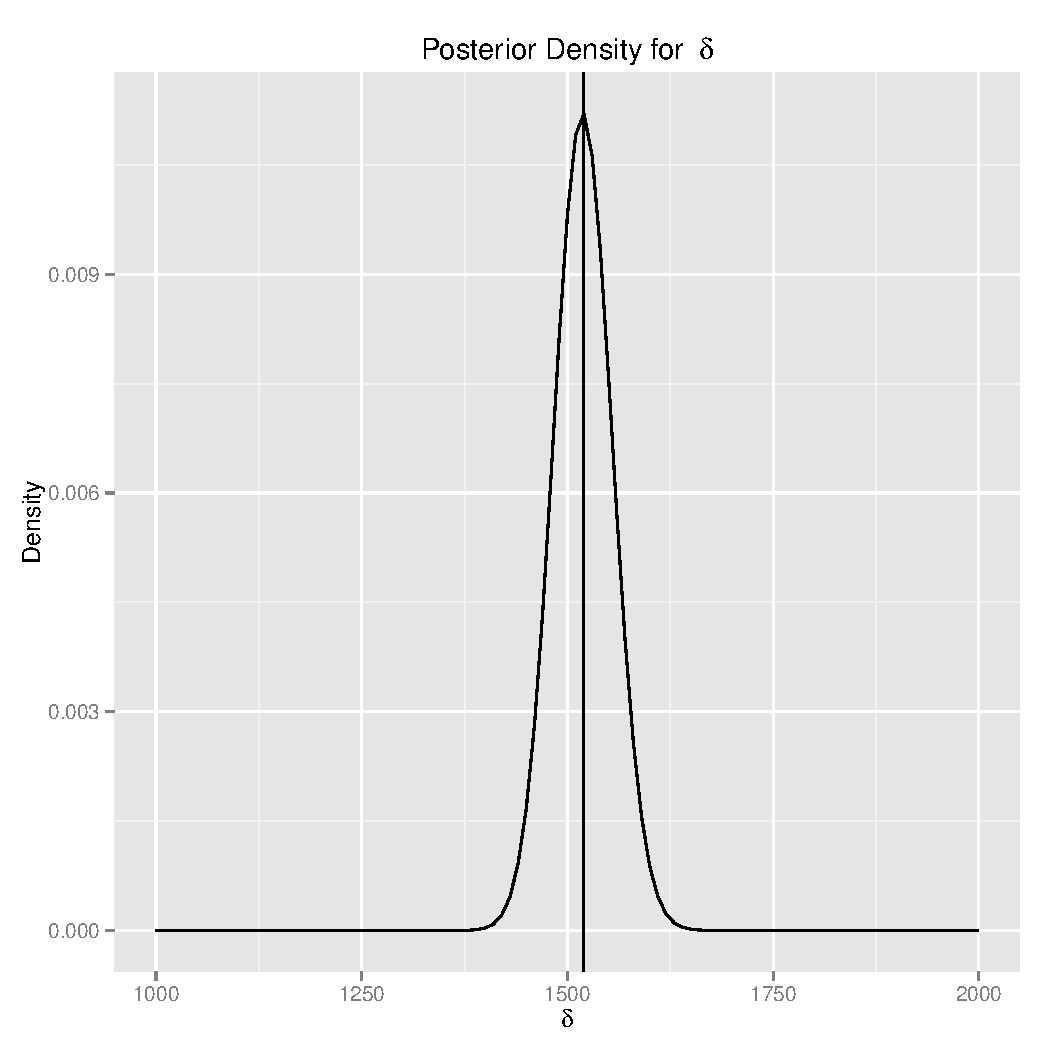
\includegraphics[width=0.85\textwidth]{delta.pdf}
    \caption{Posterior Density of $\delta$}
    \label{delta}
  \end{figure}
  \begin{figure}
    \centering
    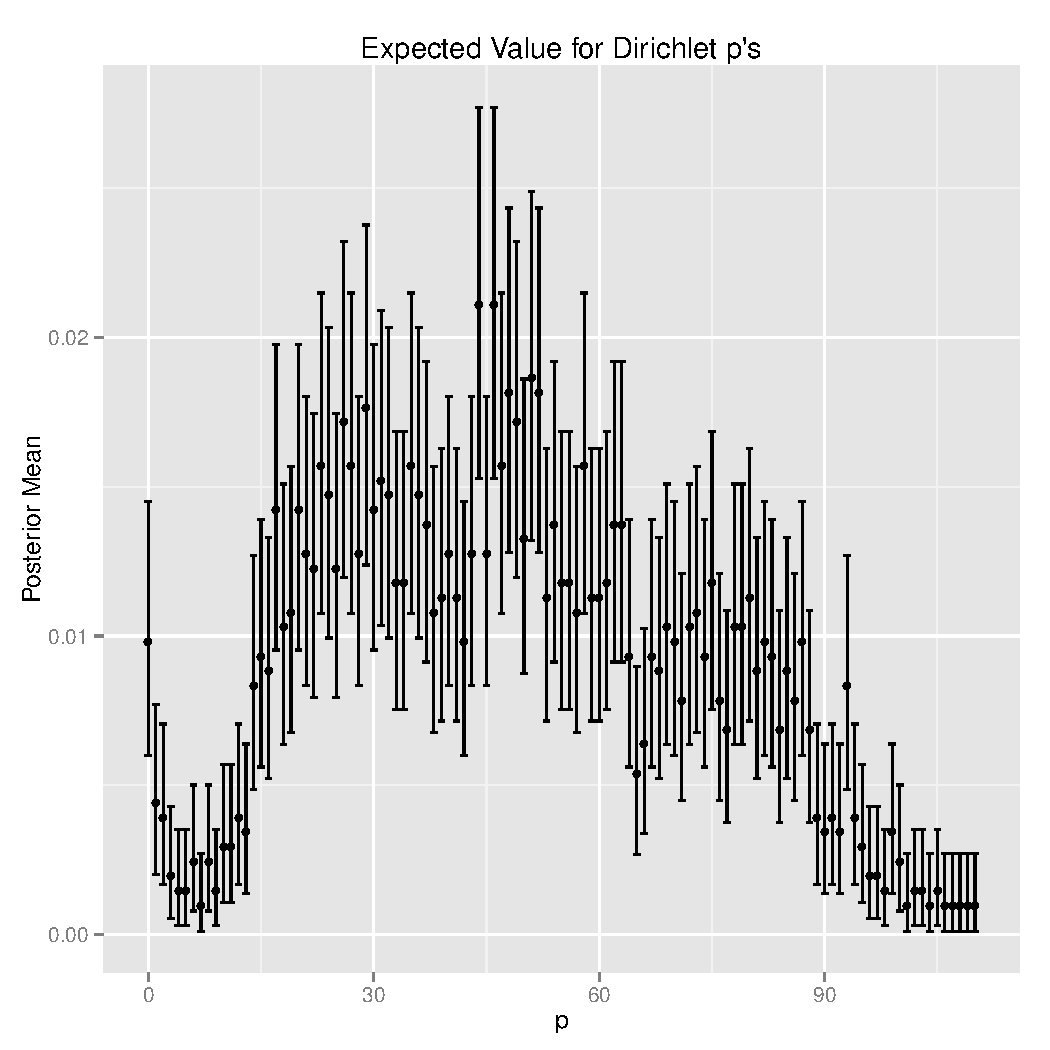
\includegraphics[width=0.85\textwidth]{dirichlet.pdf}
    \caption{Means for $p_0, \dots, p_{110}$}
    \label{dirichlet}
  \end{figure}

\end{enumerate}


\end{document}
